\chapter{Algebraic Graph Theory}%
\label{chap:09}

\paragraph*{Summary} In this lecture we discuss a unified framework that allows
to us to understand many different path problems (shortest paths, widest paths,
existence of paths etc.) in a single context. This will be done by generalising
the notion of matrix multiplications which will allow us to write shortest path,
widest path and path existence problems in terms of matrix powers.

\section{Generic Single Source Shortest Paths}
Recall again Dijkstra's algorithm. In the inner loop we look at each edge
$e = (v,u)$ in the forward star of the current looked-at node $v$. We discussed
two different types of Dijkstra's algorithm that only differ in the way the
distance $d(u)$ from the starting vertex is updated (sum of all edge weights in
shortest path; single most expensive edge weight in minimax path). We now
discuss a third variant.  Here, we want to answer the question whether or not
there is a path at all. However, this is a special case of the above discussed
methods where we encode the edges of the original path as $0$ if there is a
connection between the nodes and $\infty$ if there is no edge between two
vertices. Alternatively, we can formulate this problem as follows. Consider a
fully connected graph with edge weights $\{\mathtt{FALSE},\mathtt{TRUE}\}$. In
the initialisation phase of Dijkstra's algorithm, we set
\begin{equation*}
  d(s) = \mathtt{TRUE} \quad \text{ and } \quad d(u \in V \setminus \{s\}) = \mathtt{FALSE}\,.
\end{equation*}
The update of the ``distance'' $d(u)$ then looks as follows
\begin{equation*}
  d(u) = \mathtt{OR}(d(u),\, \mathtt{AND}(d(v), w(e)))\,.
\end{equation*}
In other words: along a path, each single edge weight has to be \texttt{TRUE}
(this is the inner \texttt{AND}) while of many different paths only one has to
be \texttt{TRUE} (this is the outer \texttt{OR}) for $d(u)$ to be set to
\texttt{TRUE}. Example applications for this problem are
\begin{itemize}
\item In computer vision this is often used when training a network that is
  supposed to detect some feature and one wants to collect all pixels that are
  connected (and lie above a certain threshold). This is usually not done using
  the approach introduced above but it the problem itself can still be solved by
  an algorithm that falls in this general framework discussed in the following.
\item Other problems include: reachability, percolation (simulate if water will
  reach the bottom when flowing through a certain network), connectedness or
  maze solving.
\end{itemize}
We see that all the different kinds of Dijkstra's algorithm are only certain
special cases of a generic single-source generalised-shortest-distance algorithm
that can find shortest and widest path as well as determine whether or not there
is a path at all etc. Note, however, that these algorithms need not be the most
efficient ones solving the particular problem (\eg for the problem of finding if
there exists a path one would implement the algorithm using a disjoint-set/
union-find data structure where each node is mapped to an index such that nodes
with same index are connected).

In 1D there is simple $\mathcal{O}(N)$ algorithm to determine whether or not two
nodes are connected. Consider the following simple graph.  \vspace*{2em}
\begin{figure}[h!]
  \centering
  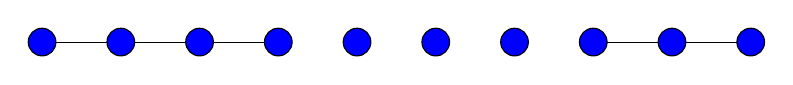
\begin{tikzpicture}
    \def\ax{1}; \def\bx{2}; \def\cx{3}; \def\dx{4}; \def\ex{5}; \def\fx{6};
    \def\gx{7}; \def\hx{8}; \def\ix{9}; \def\jx{10};

    \node (A) at (\ax,0) {}; \node (B) at (\bx,0) {}; \node (C) at (\cx,0) {};
    \node (D) at (\dx,0) {}; \node (E) at (\ex,0) {}; \node (F) at (\fx,0) {};
    \node (G) at (\gx,0) {}; \node (H) at (\hx,0) {}; \node (I) at (\ix,0) {};
    \node (J) at (\jx,0) {};

    \draw[-] (A) -- (B) -- (C) -- (D); \draw[-] (H) -- (I) -- (J);
    
    \draw[fill=blue] (A) circle (5pt); \draw[fill=blue] (B) circle (5pt);
    \draw[fill=blue] (C) circle (5pt); \draw[fill=blue] (D) circle (5pt);
    \draw[fill=blue] (E) circle (5pt); \draw[fill=blue] (F) circle (5pt);
    \draw[fill=blue] (G) circle (5pt); \draw[fill=blue] (H) circle (5pt);
    \draw[fill=blue] (I) circle (5pt); \draw[fill=blue] (J) circle (5pt);
  \end{tikzpicture}
\end{figure}

We now start from the left and assign an arbitrary label to the first node. If
the next node is connected to the current node then we assign to it the same
label. Otherwise we choose a different label. Using numbers as labels, our graph
from above might then look like this.  \vspace*{2em}
\begin{figure}[h!]
  \centering
  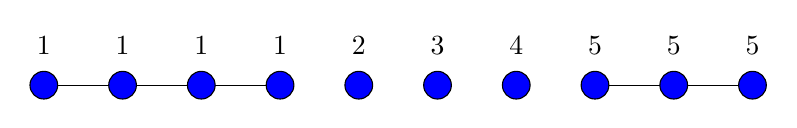
\begin{tikzpicture}
    \def\ax{1}; \def\bx{2}; \def\cx{3}; \def\dx{4}; \def\ex{5}; \def\fx{6};
    \def\gx{7}; \def\hx{8}; \def\ix{9}; \def\jx{10};

    \node (A) at (\ax,0) {}; \node (B) at (\bx,0) {}; \node (C) at (\cx,0) {};
    \node (D) at (\dx,0) {}; \node (E) at (\ex,0) {}; \node (F) at (\fx,0) {};
    \node (G) at (\gx,0) {}; \node (H) at (\hx,0) {}; \node (I) at (\ix,0) {};
    \node (J) at (\jx,0) {};

    \draw[-] (A) -- (B) -- (C) -- (D); \draw[-] (H) -- (I) -- (J);
    
    \draw[fill=blue] (A) circle (5pt); \draw[fill=blue] (B) circle (5pt);
    \draw[fill=blue] (C) circle (5pt); \draw[fill=blue] (D) circle (5pt);
    \draw[fill=blue] (E) circle (5pt); \draw[fill=blue] (F) circle (5pt);
    \draw[fill=blue] (G) circle (5pt); \draw[fill=blue] (H) circle (5pt);
    \draw[fill=blue] (I) circle (5pt); \draw[fill=blue] (J) circle (5pt);

    \def\ty {0.5}; \node at (\ax,\ty) {1}; \node at (\bx,\ty) {1}; \node at
    (\cx,\ty) {1}; \node at (\dx,\ty) {1}; \node at (\ex,\ty) {2}; \node at
    (\fx,\ty) {3}; \node at (\gx,\ty) {4}; \node at (\hx,\ty) {5}; \node at
    (\ix,\ty) {5}; \node at (\jx,\ty) {5};
  \end{tikzpicture}
\end{figure}
Checking if two nodes are connected is now simply achieved by checking whether
or not their assigned node labels are the same. Assigning the node labels is
obviously in $\mathcal{O}(N)$, where $N$ is the number of nodes and checking two
nodes is in $\mathcal{O}(1)$.

\section{All-Pairs Shortest Paths and the Distance Product}
Consider the following graph and its associated adjacency matrix.
\begin{figure}[h!]
  \centering
  \begin{tikzpicture}
    \node (A) at (0,0) {}; \node (B) at (2,1) {}; \node (C) at (2,-1) {}; \node
    (D) at (4,0) {};

    \node[circle, draw=black, fill=white, inner sep=0pt,minimum size=10pt] at
    (A) {$a$}; \node[circle, draw=black, fill=white, inner sep=0pt,minimum
    size=10pt] at (B) {$b$}; \node[circle, draw=black, fill=white, inner
    sep=0pt,minimum size=10pt] at (C) {$c$}; \node[circle, draw=black,
    fill=white, inner sep=0pt,minimum size=10pt] at (D) {$d$};

    \draw (A) -- node[above] {$7$} (B); \draw (A) -- node[below] {$1$} (C);
    \draw (C) -- node[below] {$2$} (D); \draw (B) -- node[above] {$1$} (D);
    \draw (B) -- node[right] {$5$} (C);

    \node (M) at (8,0) {%
      $A = \kbordermatrix{
        & a & b & c & d \\
        a & 0 & 7 & 1 & \infty \\
        b & 7 & 0 & 5 & 1 \\
        c & 1 & 5 & 0 & 2 \\
        d & \infty & 1 & 2 & 0 }$};
  \end{tikzpicture}
\end{figure}
where the entries $(a,d)$ and $(d,a)$ are set to $\infty$ since there is no
connection between these two vertices. Now, recall that usual matrix
multiplication formula. If we multiply two matrices $C = AB$, we have
\begin{equation*}
  {[C]}_{ij} = {\color{green}\sum_k} {[A]}_{ik} {\color{red}\cdot} {[B]}_{kj}\,.
\end{equation*}
We will now define different kinds of ``matrix multiplications'' where we
replace at least one of the sum (green) and product (red). We start by replacing
the sum by taking a minimum and replacing the product by a sum. The resulting
operation looks as follows.
\begin{equation*}
  {[C]}_{ij} = {\color{green}\min_k} {[A]}_{ik} {\color{red}+} {[B]}_{kj}\,.
\end{equation*}
If we compute the ``matrix product'' $A \cdot A$ for the adjacency matrix from
the example above using this formula we obtain
\begin{equation*}
  A^2 =
  \begin{bmatrix}    
    0 & 7 & 1 & \infty \\
    7 & 0 & 5 & 1 \\
    1 & 5 & 0 & 2 \\
    \infty & 1 & 2 & 0
  \end{bmatrix}
  \begin{bmatrix}    
    0 & 7 & 1 & \infty \\
    7 & 0 & 5 & 1 \\
    1 & 5 & 0 & 2 \\
    \infty & 1 & 2 & 0
  \end{bmatrix}
  =
  \begin{bmatrix}    
    0 & \colorbox{yellow}{6} & 1 & \colorbox{yellow}{3} \\
    \colorbox{yellow}{6} & 0 & \colorbox{yellow}{3} & 1 \\
    1 & \colorbox{yellow}{3} & 0 & 2 \\
    \colorbox{yellow}{3} & 1 & 2 & 0
  \end{bmatrix}\,.
\end{equation*}
The matrix $A$ obviously contains the cost to go from one node to another with
at most one hop. The matrix $A^2$, computed using the min sum matrix product now
contains the cost of the shortest path from all nodes to all other nodes with at
most two hops! The entries with the yellow background in the matrix above
correspond to paths where in two hops we found a shorter path as compared to
using just one hop.\footnote{This is in essence a matrix formulation of the
  Floyd-Warshal algorithm.}

If we now multiply this result again by $A$, \ie if we compute $A \cdot A^2$, we
obtain the cheapest cost from all nodes to all other nodes while taking at most
three hops. The result is as follows
\begin{equation*}
  AA^2 =
  \begin{bmatrix}    
    0 & 7 & 1 & \infty \\
    7 & 0 & 5 & 1 \\
    1 & 5 & 0 & 2 \\
    \infty & 1 & 2 & 0
  \end{bmatrix}
  \begin{bmatrix}    
    0 & {6} & 1 & {3} \\
    {6} & 0 & {3} & 1 \\
    1 & {3} & 0 & 2 \\
    {3} & 1 & 2 & 0
  \end{bmatrix}
  =
  \begin{bmatrix}    
    0 & \colorbox{yellow}{4} & 1 & {3} \\
    \colorbox{yellow}{4} & 0 & {3} & 1 \\
    1 & {3} & 0 & 2 \\
    {3} & 1 & 2 & 0
  \end{bmatrix}\,.
\end{equation*}
We again highlighted the costs that have changed. If repeat this process another
time, the matrix no longer changes since in a graph with four nodes, we can only
do three hops before arriving at nodes that have been visited on the
path. Depending on the graph, this ``convergence'' might happen earlier.

We can use this iterated generalised matrix multiplication to also solve minimax
path and path-existence problems that we have discussed earlier. For the minimax
path we define the matrix product as
\begin{equation*}
  {[C]}_{ij} = {\color{green}\min_k}\ {\color{red}\max\Big\{}{[A]}_{ik} {[B]}_{kj}{\color{red}\Big\}}\,.
\end{equation*}
Again using the example from the beginning of the section, after two hops we
have
\begin{equation*}
  A^2 =
  \begin{bmatrix}    
    0 & 7 & 1 & \infty \\
    7 & 0 & 5 & 1 \\
    1 & 5 & 0 & 2 \\
    \infty & 1 & 2 & 0
  \end{bmatrix}
  \begin{bmatrix}    
    0 & 7 & 1 & \infty \\
    7 & 0 & 5 & 1 \\
    1 & 5 & 0 & 2 \\
    \infty & 1 & 2 & 0
  \end{bmatrix}
  =
  \begin{bmatrix}    
    0 & \colorbox{yellow}{5} & 1 & \colorbox{yellow}{2} \\
    \colorbox{yellow}{5} & 0 & \colorbox{yellow}{2} & \colorbox{yellow}{1} \\
    1 & \colorbox{yellow}{2} & 0 & 2 \\
    \colorbox{yellow}{2} & 1 & 2 & 0
  \end{bmatrix}\,,
\end{equation*}
and after three hops
\begin{equation*}
  AA^2 =
  \begin{bmatrix}    
    0 & 7 & 1 & \infty \\
    7 & 0 & 5 & 1 \\
    1 & 5 & 0 & 2 \\
    \infty & 1 & 2 & 0
  \end{bmatrix}
  \begin{bmatrix}    
    0 & {5} & 1 & {2} \\
    {5} & 0 & {2} & {1} \\
    1 & {2} & 0 & 2 \\
    {2} & 1 & 2 & 0
  \end{bmatrix}\,, =
  \begin{bmatrix}    
    0 & \colorbox{yellow}{2} & 1 & 2 \\
    \colorbox{yellow}{2} & 0 & {1} & {2} \\
    1 & {2} & 0 & 2 \\
    {2} & 1 & 2 & 0
  \end{bmatrix}\,.
\end{equation*}
Again, the result after four hops is the same as after three.  Lastly, for the
path existence problem we let
\begin{equation*}
  {[C]}_{ij} = {\color{green}
    \underset{k}{\texttt{OR}\,}
  }
  {\color{green}\Big\{}
  {[A]}_{ik} {\color{red}\texttt{ AND }} {[B]}_{kj}
  {\color{green}\Big\}}\,.
\end{equation*}
As mentioned above, the edge weights are now either \texttt{T} = \texttt{TRUE}
or \texttt{F} = \texttt{FALSE} depending on whether or not an edge connects the
two nodes in consideration. Thus the matrix after one hop is given by
\newcommand{\TRUE}{\mathtt{T}} \newcommand{\FALSE}{\mathtt{F}}
\begin{equation*}
  A=
  \begin{bmatrix}
    \TRUE & \TRUE & \TRUE & \FALSE \\
    \TRUE & \TRUE & \TRUE & \TRUE \\
    \TRUE & \TRUE & \TRUE & \TRUE \\
    \FALSE & \TRUE & \TRUE & \TRUE \\
  \end{bmatrix}\,.
\end{equation*}
The result after two hops is then given by
\begin{equation*}
  A^2 =
  \begin{bmatrix}
    \TRUE & \TRUE & \TRUE & \FALSE \\
    \TRUE & \TRUE & \TRUE & \TRUE \\
    \TRUE & \TRUE & \TRUE & \TRUE \\
    \FALSE & \TRUE & \TRUE & \TRUE \\
  \end{bmatrix}
  \begin{bmatrix}
    \TRUE & \TRUE & \TRUE & \FALSE \\
    \TRUE & \TRUE & \TRUE & \TRUE \\
    \TRUE & \TRUE & \TRUE & \TRUE \\
    \FALSE & \TRUE & \TRUE & \TRUE \\
  \end{bmatrix}
  =
  \begin{bmatrix}
    \TRUE & \TRUE & \TRUE & \colorbox{yellow}{\texttt{T}} \\
    \TRUE & \TRUE & \TRUE & \TRUE \\
    \TRUE & \TRUE & \TRUE & \TRUE \\
    \colorbox{yellow}{\texttt{T}} & \TRUE & \TRUE & \TRUE \\
  \end{bmatrix}\,,
\end{equation*}
after which the result obviously does not change anymore. Note that we can speed
the method up by using the fact that after we have computed $A^2 = A \cdot A$ we
can use this to compute $A^4 = A^2 \cdot A^2$ etc. In practice one would also
use optimised matrix multiplication algorithms and/ or use approximations of the
matrices (\eg one might only use randomly selected rows and columns).

Note that we did consider all-pairs path problems. In practice one does often
not have enough memory to store this matrix and thus, instead of applying these
algorithms to the original image, they are applied to patches or superpixels.

\section{The Algebraic Path Problem}
We have just seen that single source (generalised Bellmann-Ford) and all pairs
shortest paths (generalised Floyd-Warshall, distance matrix product) algorithms
can be seen as special cases of one basic algorithm. More precisely, they can be
seen as multiple incarnations of matrix multiplications on different
\emph{commutative semirings}.  We start with a short recap on monoids.

\begin{definition*}
  A \emph{monoid} $(\K, \boldsymbol{\cdot}, \overline{e})$ is a set $\K$ with a
  binary operation $\boldsymbol{\cdot} : \K \times \K \rightarrow \K$ such that
  for all $a,b,c \in \K$, the equation
  \begin{equation*}
    (a \boldsymbol{\cdot} b) \boldsymbol{\cdot} c = a \boldsymbol{\cdot} (b \boldsymbol{\cdot} c)
  \end{equation*}
  holds and an identity element $\overline{e}$ which satisfies
  \begin{equation*}
    a \boldsymbol{\cdot} \overline{e} = \overline{e} \boldsymbol{\cdot} a\,, \quad \text{for all } a \in \K\,.
  \end{equation*}
  If additionally we have $a\boldsymbol{\cdot}b = b \boldsymbol{\cdot} a$ for
  all $a,b \in \K$ we call the monoid \emph{commutative}.
\end{definition*}
We can now define a semiring.
\begin{definition*}
  A semiring is a system $(\K,\oplus,\otimes,\overline{0},\overline{1})$ such
  that
  \begin{enumerate}
  \item $(\K, \oplus, \overline{0})$ is a commutative monoid,
  \item $(\K, \otimes, \overline{1})$ is a monoid (not necessarily commutative),
  \item $\otimes$ distributes over $\oplus$, \ie for all $a,b,c \in \K$ we have
    \begin{align*}
      (a \oplus b) \otimes c &= (a \otimes c) \oplus (b \otimes c) \\
      c \otimes (a \oplus b) &= (c \otimes a) \oplus (c \otimes b)\,,
    \end{align*}
    and
  \item $\overline{0}$ is an annihilator for $\otimes$, \ie
    $a \otimes \overline{0} = \overline{0} \otimes a = \overline{0}$ for all
    $a \in \K$.
  \end{enumerate}
  The semiring is said to be commutative is $\otimes$ is commutative.
\end{definition*}
Given a semiring, one can define the associated matrix semiring $M_n(\K)$ of
$n \times n$ matrices with entries in $\K$. Note that commutativity does not
necessarily transfer from $\K$ to $M_n(\K)$.  This is what we essentially used
in the previous section where we discussed different matrix semirings such as
the minmax semiring.

We now consider the algebraic path problem. We begin with the following equation
that defines the entries of a distance matrix ${[D]}_{st}$ from a source $s$ to
a target $t$ as
\begin{equation*}
  {[D]}_{st} = \bigoplus_{P \in \mathcal{P}_{st}} \bigotimes_{e \in P} w_e\,,
\end{equation*}
where $\mathcal{P}_{st}$ is the set of all paths $P$ from $s$ to $t$ and
$\otimes$ is taken over all edges within $P$. Here $\otimes$ is the semiring
multiplication and is applied along the path whereas the semiring addition
$\oplus$ is done between paths. For instance, when we solve the shortest path
problem, we can interpret this as solving the algebraic path problem in the
$(\min, \text{sum})$ semiring.

\section{Infimal Convolution, Morphology and the Euclidean Distance Transform}
We discussed earlier that convolution can be written as a matrix multiplication
with a Toeplitz matrix. We can now define a generalised notion of convolution
similar to how we generalised matrix multiplication in the previous
section. There, we defined matrix multiplication over a semiring as
\begin{equation*}
  {[AB]}_{ij} = \bigoplus_k {[A]}_{ik} \otimes {[B]}_{kj}\,.
\end{equation*}
Analogously, one can define a generalised inner product
\begin{equation*}
  \langle a,b \rangle = \bigoplus_k a_k \otimes b_k\,.
\end{equation*}
With the same approach, we can define convolution on different semirings, \eg on
the sum-product semiring
\begin{equation*}
  f \star g(x) = \sum_y f(x-y) \cdot g(y)\,,
\end{equation*}
which results in the ``standard'' convolution that we have seen earlier or on
the min-sum semiring (also referred to as the \emph{tropical semiring})
\begin{equation*}
  f \star g(x) = \inf_y\left( f(x-y) + g(y)\right)\,,
\end{equation*}
which results in the important generalisation of the \emph{infimal} or
\emph{tropical convolution}. In the context of mathematical morphology, this
operation is often referred to as \emph{erosion}\footnote{Analogously, one can
  define the max-sum convolution which is usually called \emph{dilation}}. The
function $g$ is then usually called a \emph{structuring element} (SE). In the
figure below we plotted one row of a greyscale image together with the result
(light blue line) of the erosion using the structural element given on the
right. As we can see, the erosion computes a lower envelope of the signal. We
also observe that positive peaks shrink; more precisely, peaks that are thinner
than the structuring element disappear.  (in image analysis, we can for example
use this to pre-process images to get rid of bright speckles). Valleys and
sinks, on the other hand, are expanded. If we would apply dilation to the same
signal (with the structuring element being constant in the interval
$[-\tau, \tau]$ and zero everywhere else), we would observe the opposite
effects.

\begin{figure}[htpb]
  \centering
  \begin{subfigure}[b]{0.5\textwidth}
    \includegraphics[width=\textwidth]{Figures/tropical_convolution}
    \caption{Erosion applied to one row of a greyscale image.}
  \end{subfigure}\hspace{3em}%
  \begin{subfigure}[b]{0.3\textwidth}
    \includegraphics[width=\textwidth]{Figures/structural_element}
    \caption{Structural element that was used in the example.}
  \end{subfigure}%
  \label{fig:tropconv}%
  \caption{Example of infimal convolution.}%
\end{figure}
and dilation to obtain
\begin{equation*}
  \text{opening } \coloneqq \text{ dilation}(\text{erosion}(\text{image},\text{SE}),\text{SE}) 
\end{equation*}
and
\begin{equation*}
  \text{closing } \coloneqq \text{ erosion}(\text{dilation}(\text{image},\text{SE}),\text{SE})\,,
\end{equation*}
where SE stands for structuring element. Since erosion shrinks all objects which
leads to the elimination of small objects and dilation enlarges objects, the
opening operation can be used to get rid of very small objects in
images. Closing, on the other hand, gets rid of small holes in objects, since
these holes get first ``filled'' by the dilation operation after which erosion
than shrinks the objects to their original size, but keeping the holes
``filled''.

%%% Local Variables:
%%% mode: latex
%%% TeX-master: "../main"
%%% End:
